\documentclass[letterpaper,11pt]{article}
\usepackage{aaai}
\usepackage{times}
\usepackage{helvet}
\usepackage{courier}
\usepackage{graphicx}
\usepackage{url}
\usepackage{amssymb, amsmath}
\usepackage{subcaption}
\begin{document}

\title{Predicting Flight Delays with LAMP and a Sliding Window}
\author{\\Adrian Lim A0123432W \\
Ng Hui Xian Lynnette A0119646X \\
Toh ZiJing A0123506R }
\maketitle
\begin{abstract}
\begin{quote}
Have you ever been stuck in an airport because your flight was delayed or cancelled and wondered if you could have predicted it if you'd had more data? In this project, we used 7.5 million entries worth of commercial flight data within USA to answer the following question: Given a current flight's data and the past few days of flight data, can you predict if the flight will be delayed? The 1.04 GB of flight data is obtained from RITA, and combined with meteorological data from NOAA as well as latitude and longitude data. As per the RITA definition of delay, a flight is considered to be delayed ifs it is more than 15 minutes late. This project explores using different window sizes as the number of previous days of training data to predict a query flight. It extracts k-nearest-neighbours from the training data, where $k$ is a fraction of $n$ records of training data, before performing various classifiers on the new dataframe. Using the map-reduce architecture, this project parallizes computation with multiple mappers computing the classification label of IsDelayed and one reducer aggregating the results to formulate the precision and recall score for the parameters $n$, $k$ and the classifier.
\end{quote}
\end{abstract}

\section{Introduction}
Have you ever been stuck in an airport because your flight was delayed or cancelled and wondered if you could have predicted it if you'd had more data? ASA Statistical Computing hosted a Data Expo competition in 2009 \cite{asa_stat} on Airline on-time performance. The challenge of the Data Expo is to provide a graphical summary of the flight data consisting of flight arrival and departure details from all the commercial flights within America from October 1987 to April 2008. The dataset contains about 120 million records in total and is 12GB large. A total of nine entires were received, and many made use of tools such as R, Hadoop and Spark.

In this project, we make use of the flight data for Year 2007 and try to answer the following question: Given a current flight's data and the past few days of flight data, can you predict if the flight will be delayed? We use the RITA definition of delay, where a flight is considered to be delayed if it is more than 15 minutes late. This project explores different number of days of past data used for training (henceforth referred to as window size), and its effect on the precision and recall of classification. 

\subsection{Literature Review}
Xu \cite{Xu_1estimation} used Naive Bayes to construct a Dirichlet prior distribution in order to estimate the delay in the American national aviation system. The accuracy of their method is around 81\%. \cite{juannetwork} used Random Forest algorithms built upon temporal and spatial variables over a 2 hour prediction horizon, with an error rate of 19\%. However, they classified delays as 60 minutes and not 15 minutes as per the RITA definition. \cite{smithsvm} had approximately 83\% success rate in using Support Vector Machines (SVM) to predict the aircraft arrival rates with flight data augmented with meteorological data. 

Some student prediction projects using this dataset include Predicting Flight Delays through Data Mining\cite{bostonu}, where data from Year 2008 was used for prediction. No additional data added to the dataset, and a variety of classifiers such as the NB Tree, J48 Decision Tree, PART, Decision Table and OneR classifiers from WEKA were used on the dataset with an average prediction accuracy of 62.6\%. Stanford students Lawson and Castillo \cite{lawson} combined the dataset with NOAA weather data and performed binary classification on the dataset using Naive Bayes, Random Forest and SVM. Their best precision was 86\% with Random Forest on a selected test set from Newark Liberty International Airport. With random query flights, their average prediction accuracy is 85\%. 

\subsection{Commercial Sites}
There are commercial sites that are built to benefit passengers by predicting flight delays. For commercial flights within USA, there are two main such sites. One of them is Flightcaster, which claims a precision of 85\% and a recall of 61\%.\cite{flightcaster} Another site is KnowDelay \cite{knowdelay}, but its precision-recall rate is not reported

\section{The Data }
The flight dataset is taken from RITA, the United States Department of Transportation. For this project, we used only the data from Year 2007, which contains over 7.5 million flight records and is 1.04 GB uncompressed. Figure \ref{fig:flightdata} shows a table of the values in the data and has been colour coded with into four categories: spatial data (blue), carrier data (green), temporal data (orange) and delay statistics (yellow). 

\begin{figure}[htb]
\centering
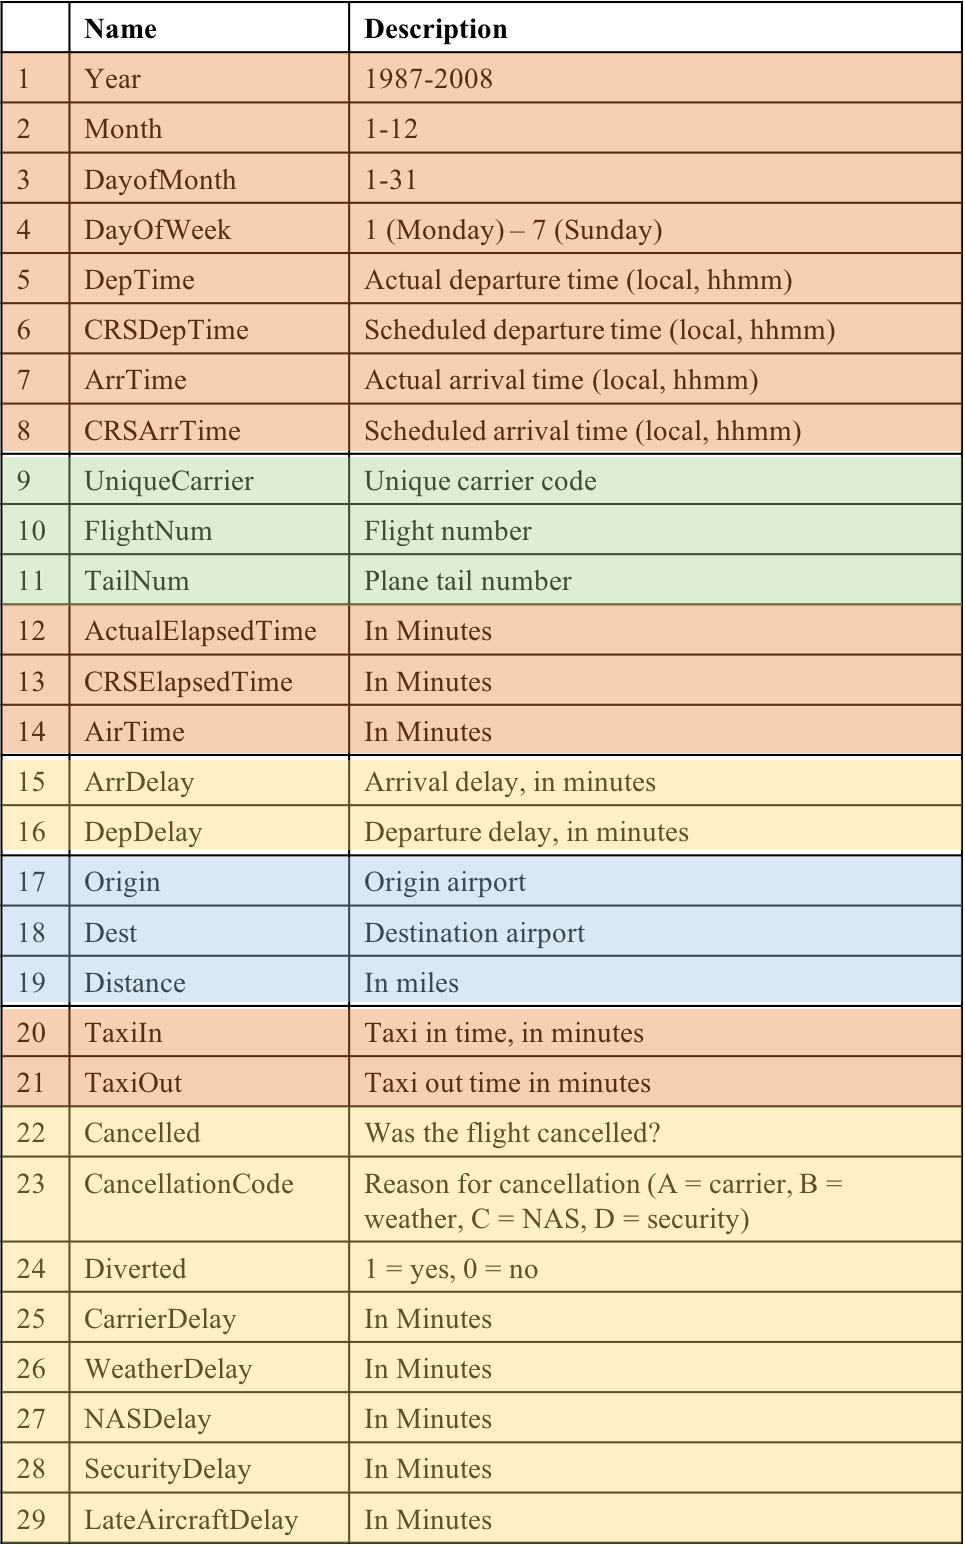
\includegraphics[height=1.2\linewidth]{flightdata.png}
\caption{Fields in the Flight Data}
\label{fig:flightdata}
\end{figure}

We combine the data with weather data from NOAA (National Oceanic and Atmospheric Administration), which provides temperature, precipitation and wind speed data collected from the various airport weather stations. Figure \ref{fig:weatherdata} shows a table of the fields in the weather data set.\\ 

\begin{figure}[htb]
\centering
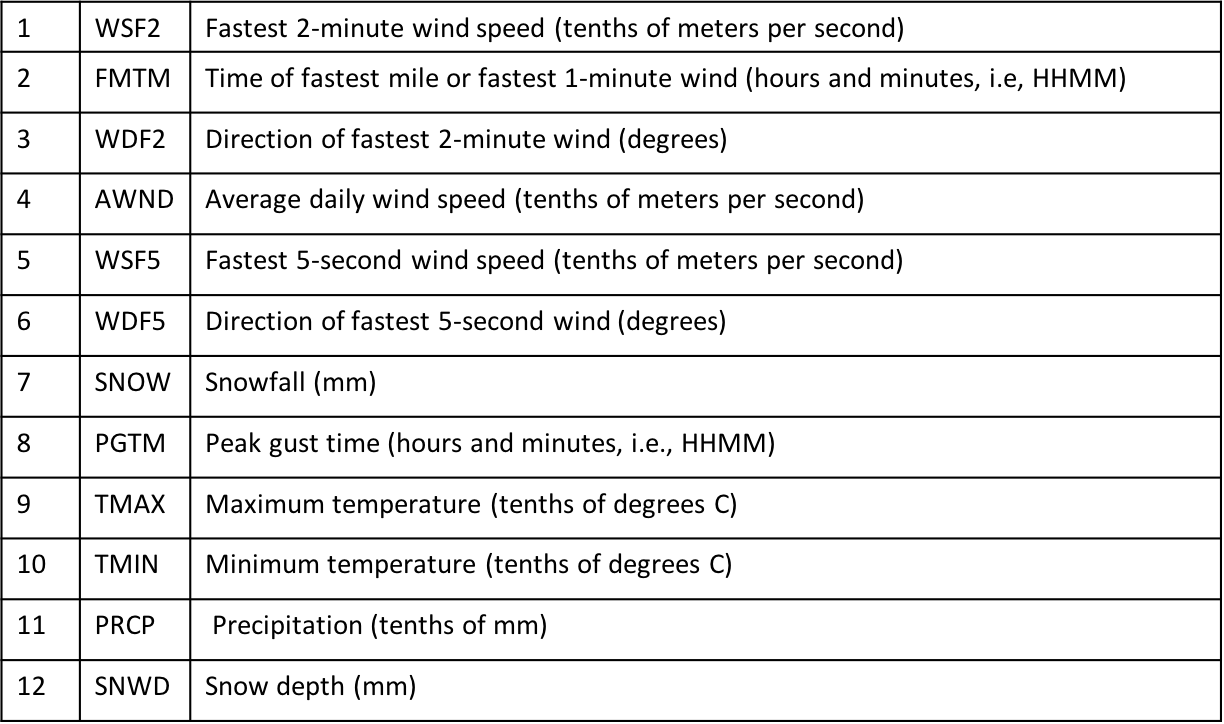
\includegraphics[height=0.6\linewidth]{weatherdata.png}
\caption{Fields in the Weather Data}
\label{fig:weatherdata}
\end{figure}

We also add data about the distances between the origin and destination airports, calculated from the latitude and longitude of the airports. 

\section{Exploratory Data Analysis}
In this section, we present certain findings and graphs generated from the raw data itself. This helps us with our feature selection in the preprocessing step. In year 2007, 2 244 514, or 30\% of the flights were considered delayed. On average, there are about 20, 407 commercial flights per day within USA. There are 5000 unique flight routes, or origin-destination pairs, a fraction of which is represented in Figure \ref{fig:flightroutes}. We also chart the percentage of delays of the airport when they are the Origin airport or Destination airports. Figure \ref{fig:airportdelays} show the 20 airports with the most number of delays, by airport code. Most are municipal airports, hence it is acceptable for them to experience high delays as they have a small land space and lesser resources yet have to still cope with the volume of inbound and outbound flights. International airports that are in this top 20 list include those with much passenger traffic, such as Atlantic City International Airport and John F Kennedy International Airport. A similar chart in Figure \ref{fig:delaybyorigin} depicts delays experienced by outbound flights and the cause of delays. 

Number of delays by Day of Week as depicted by \ref{fig:weekdelays} do not have much deviations, as the average number of delays on each day is 32 000 flights. Figure \ref{fig:heatmap} presents a star chart on the number of delays from the origin to destination airports. The lines which are most strong are generally major international airports. Some airports are Chicago O'Hare International Airport, JFK International Airport and San Francisco International Airport. 

\begin{figure}[htb]
\centering
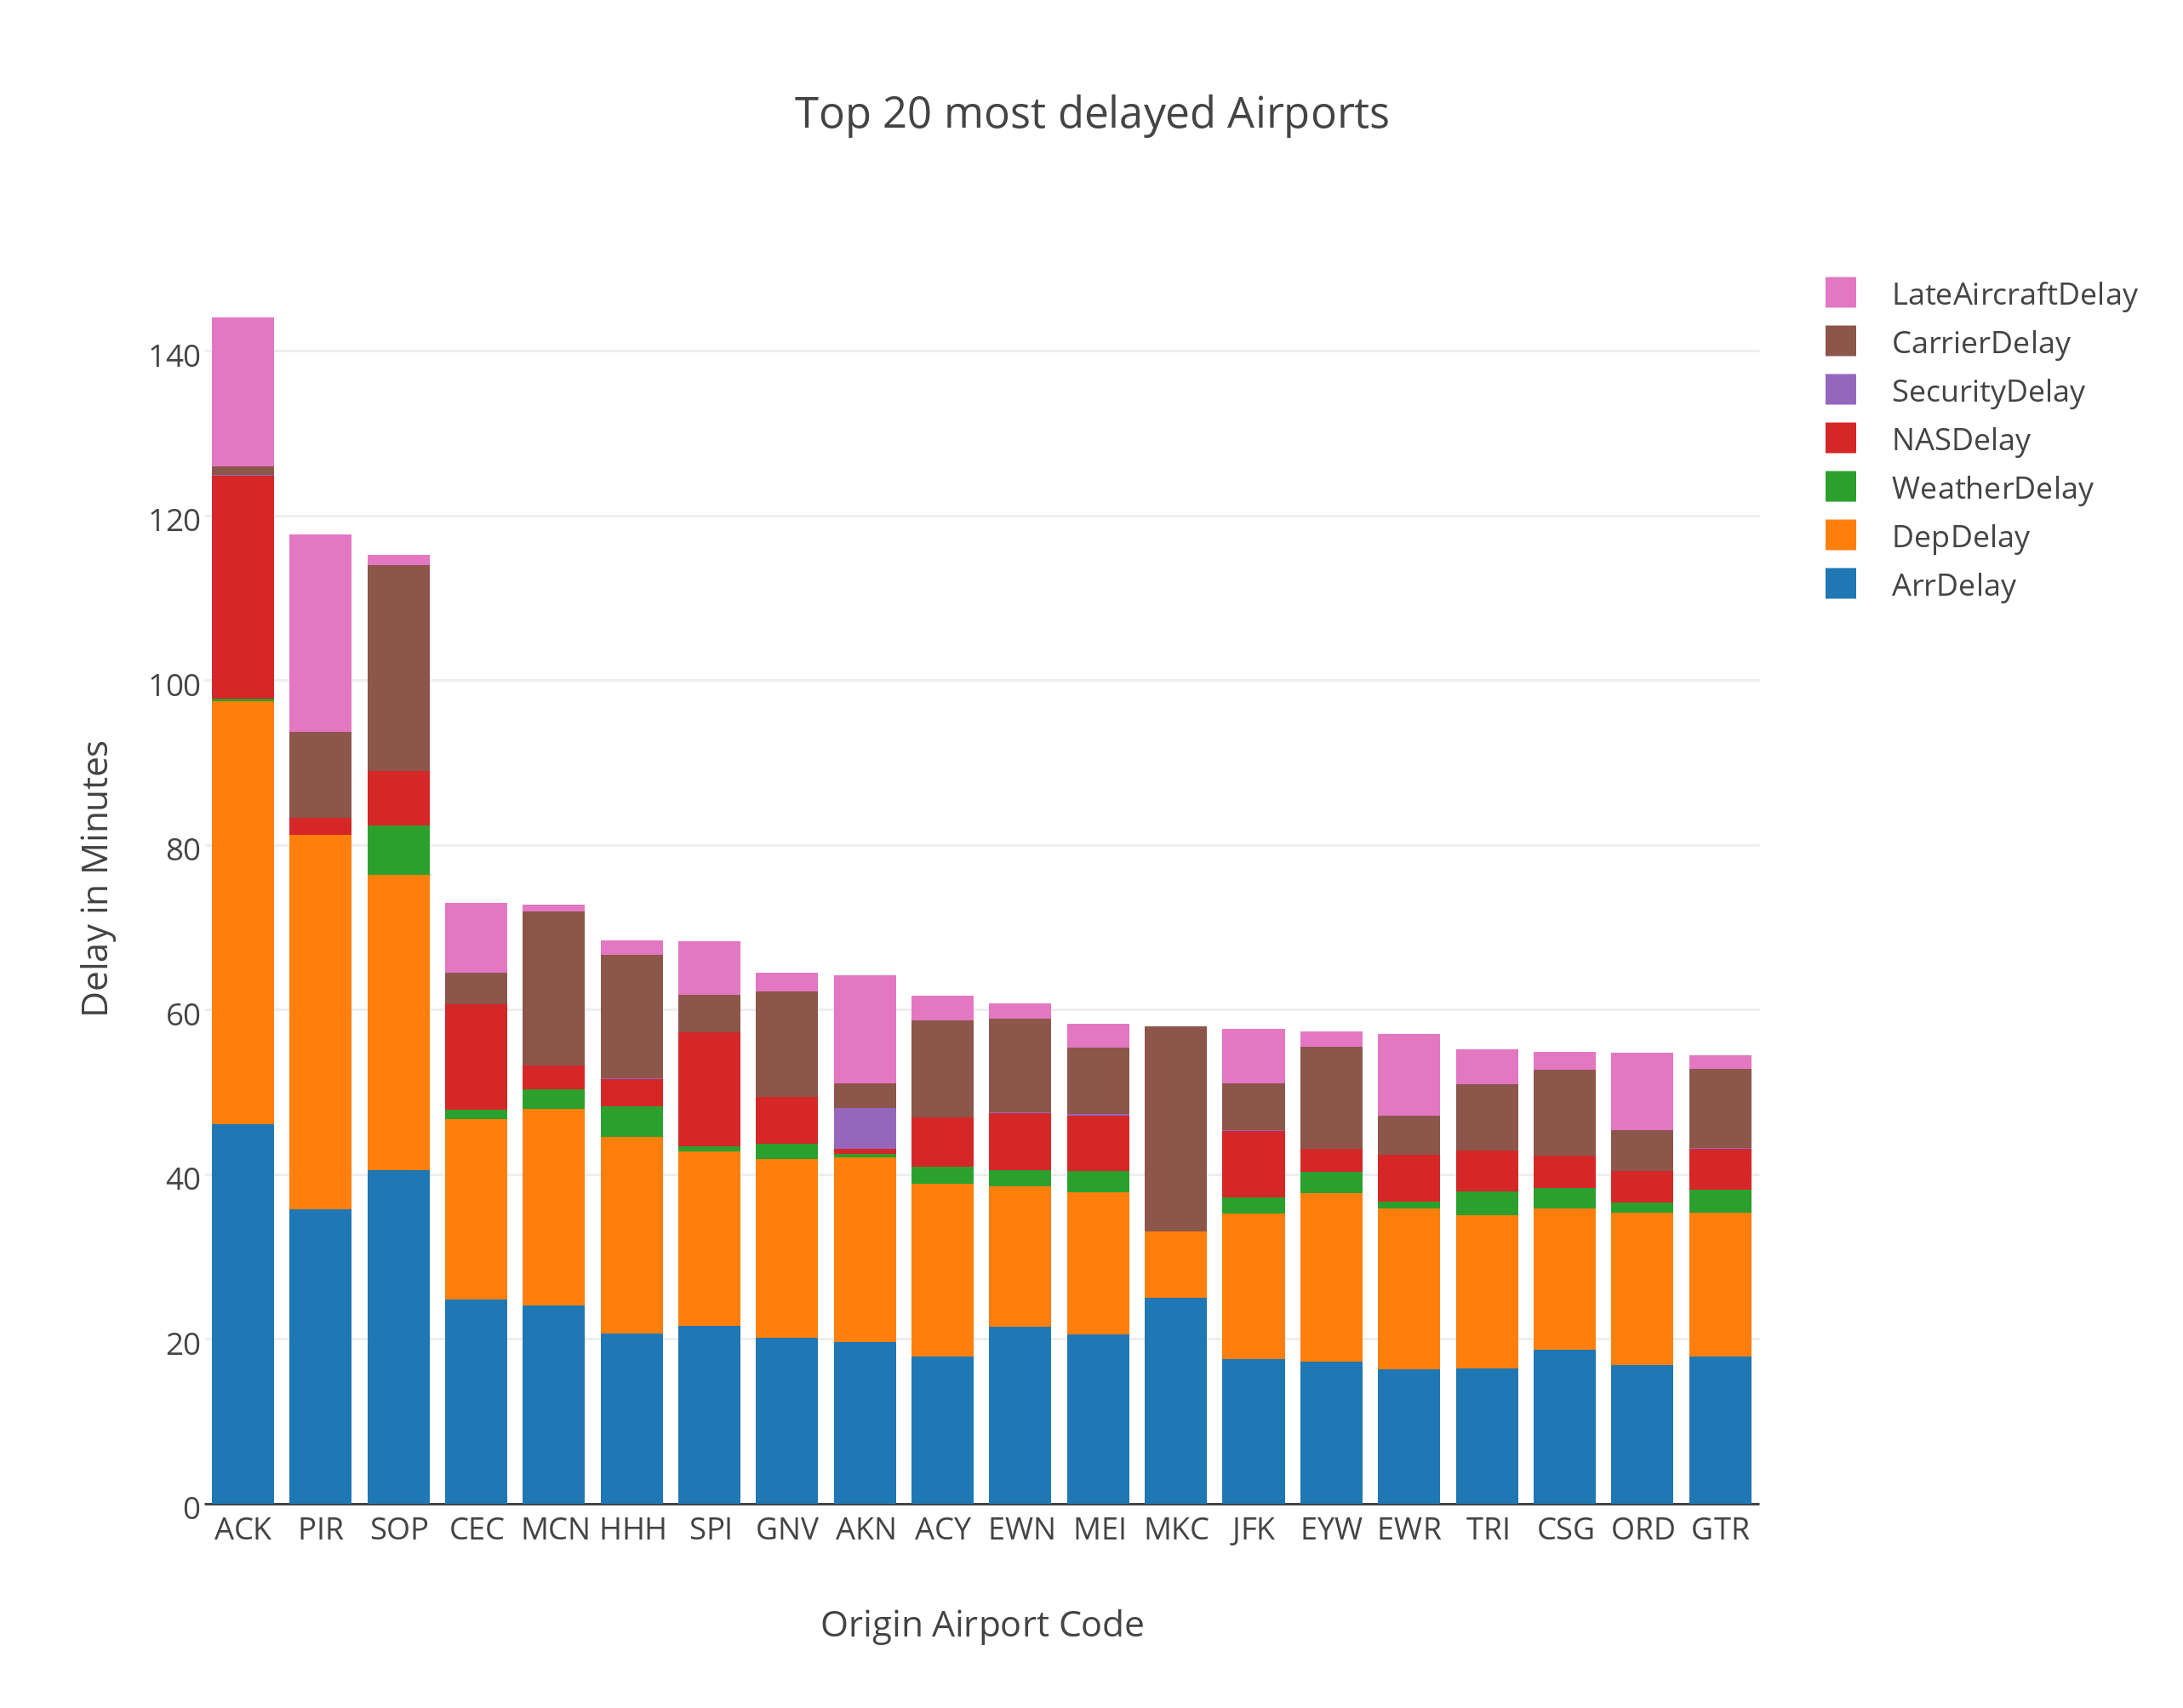
\includegraphics[width=1.1\linewidth]{delaybyorigin.png}
\caption{Chart of Delays by Origin Airports (i.e. represents outbound flights)}
\label{fig:delaybyorigin}
\end{figure}

\begin{figure}[htb]
\centering
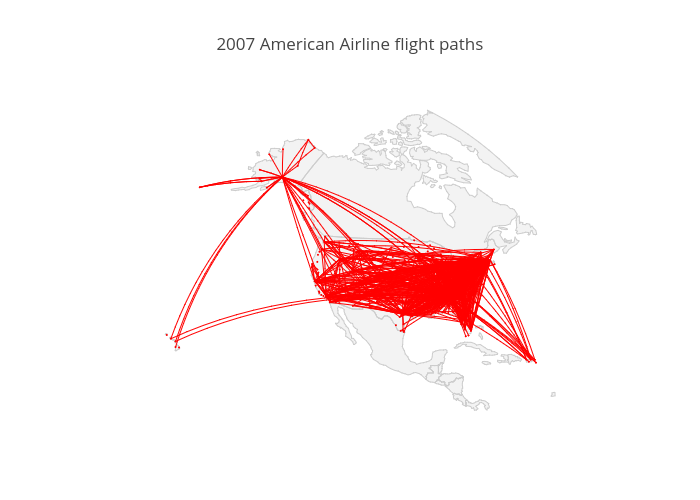
\includegraphics[width=1.1\linewidth]{airportpaths.png}
\caption{Chart of Delays by Airport}
\label{fig:flightroutes}
\end{figure}

\begin{figure}[htb]
\centering
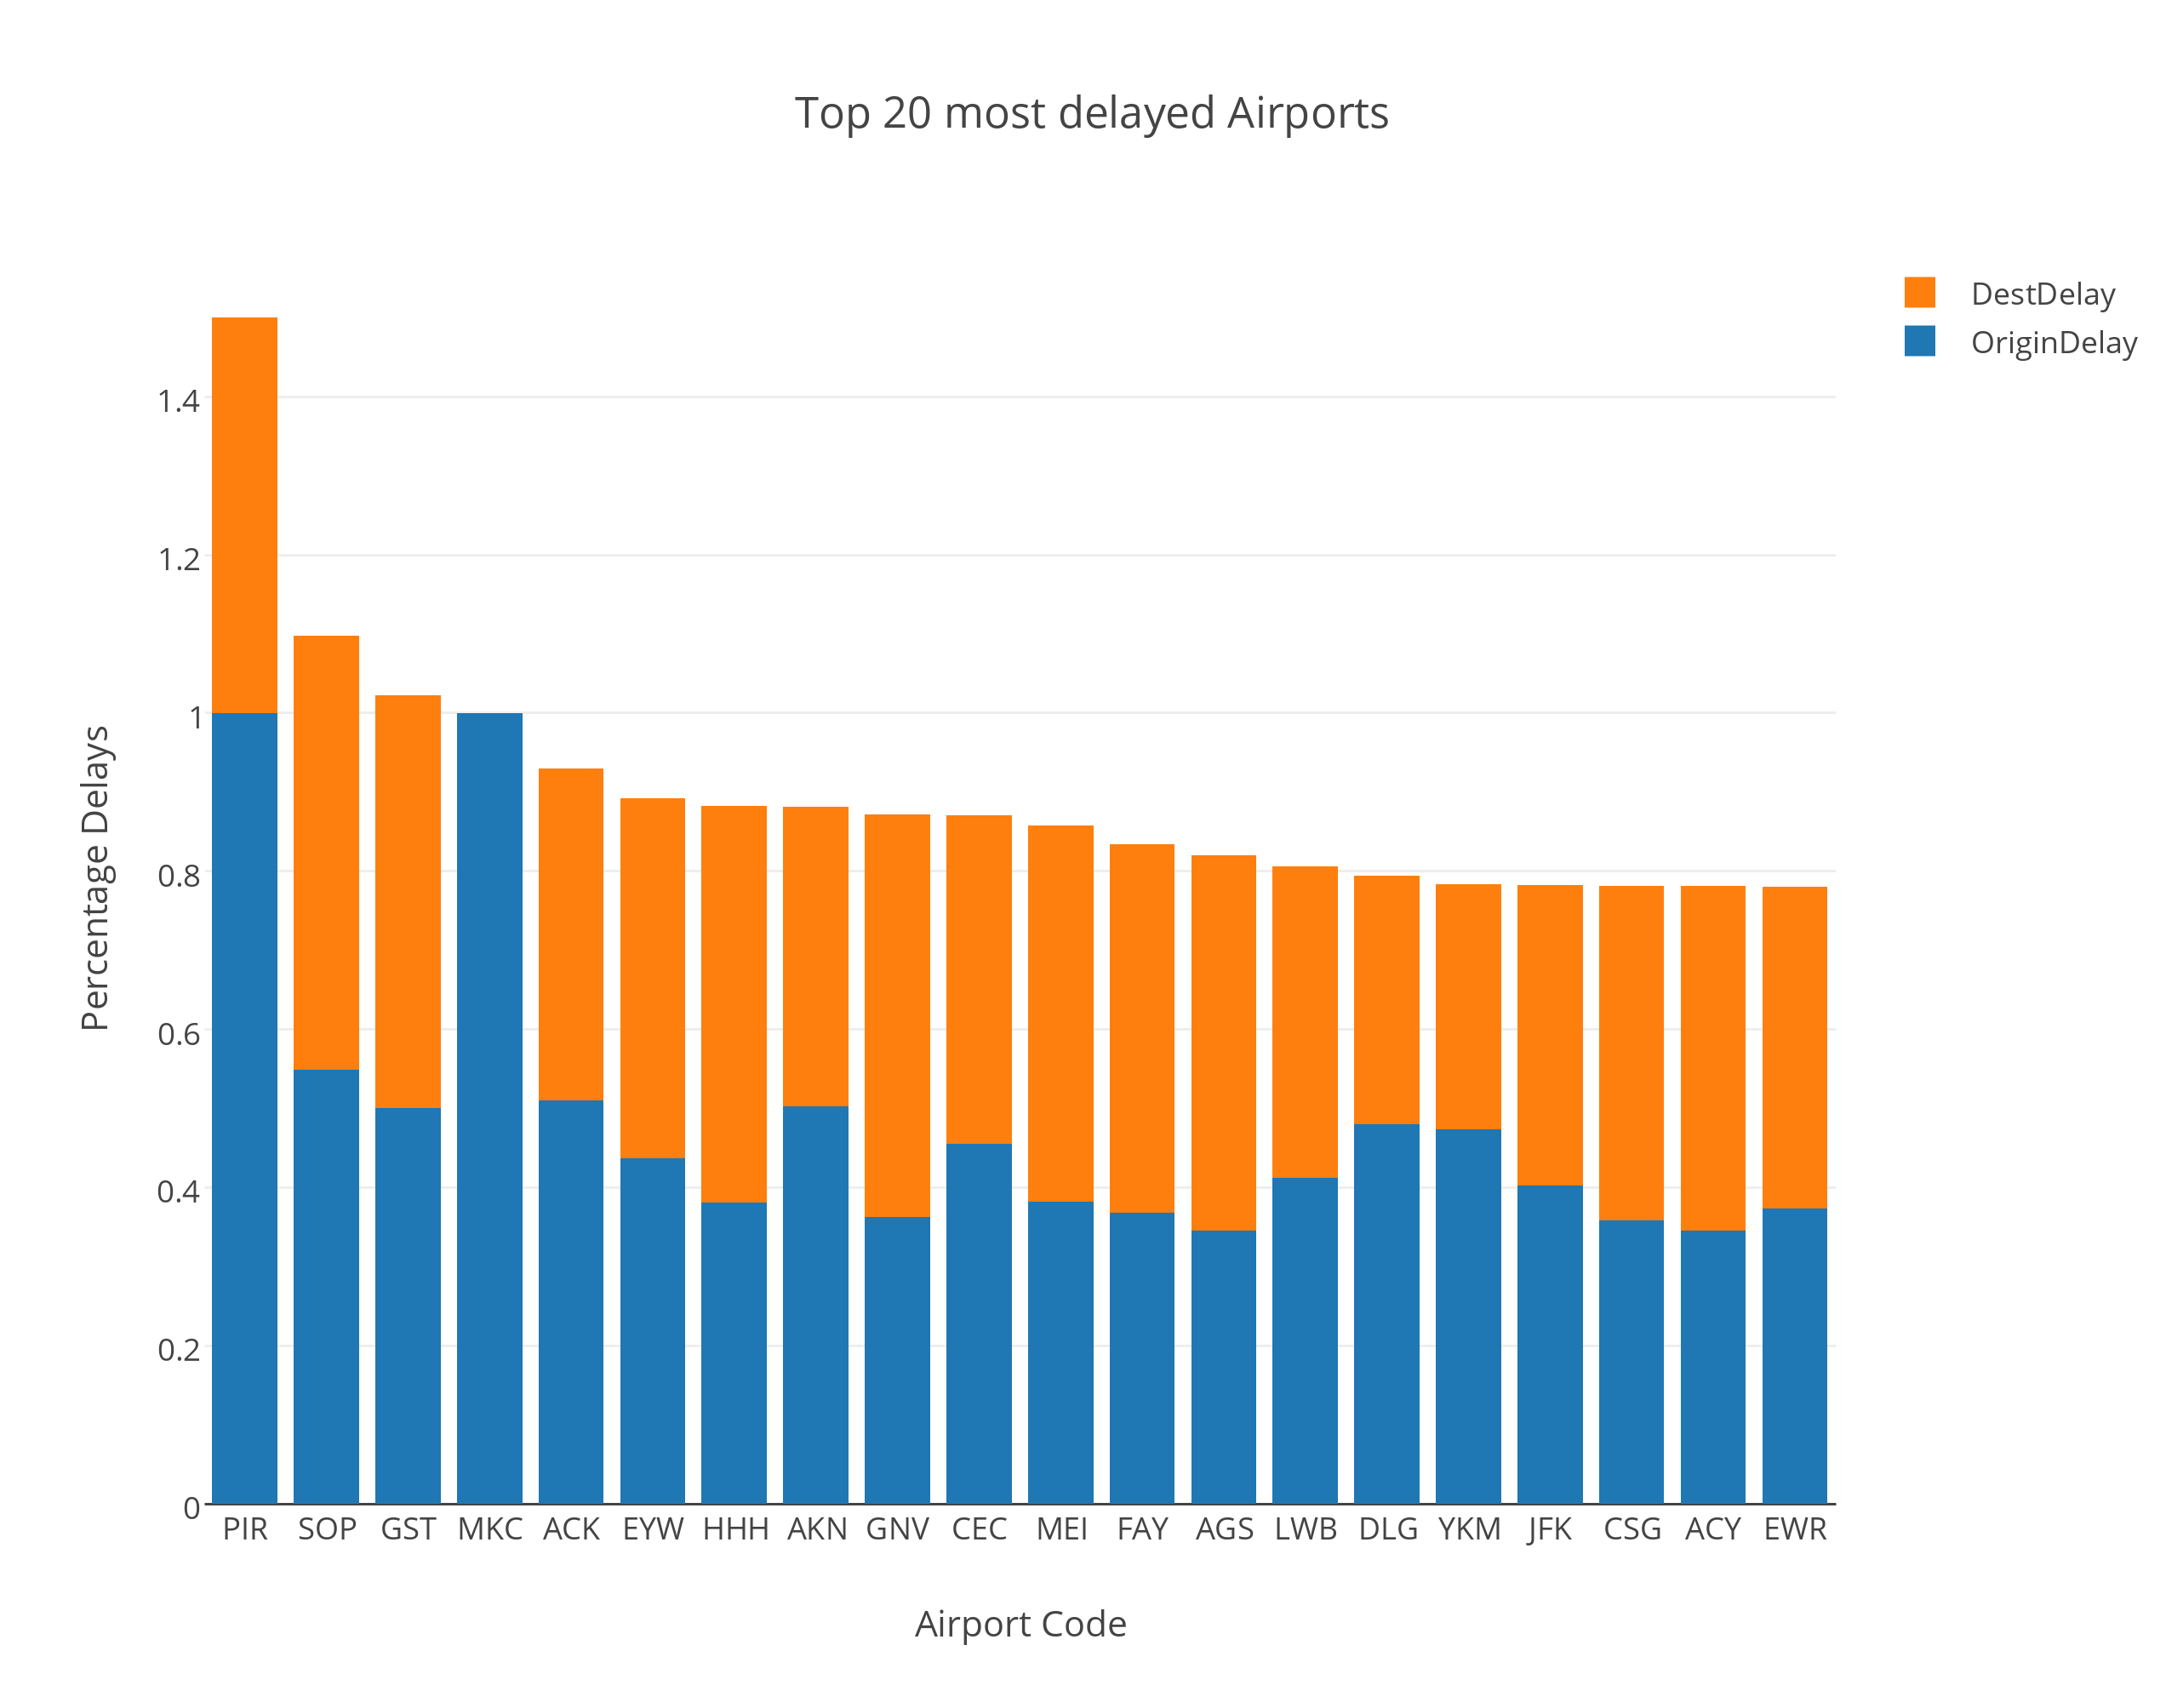
\includegraphics[width=1.1\linewidth]{delayedairports.png}
\caption{Chart of Delays by Airport}
\label{fig:airportdelays}
\end{figure}

\begin{figure}[htb]
\centering
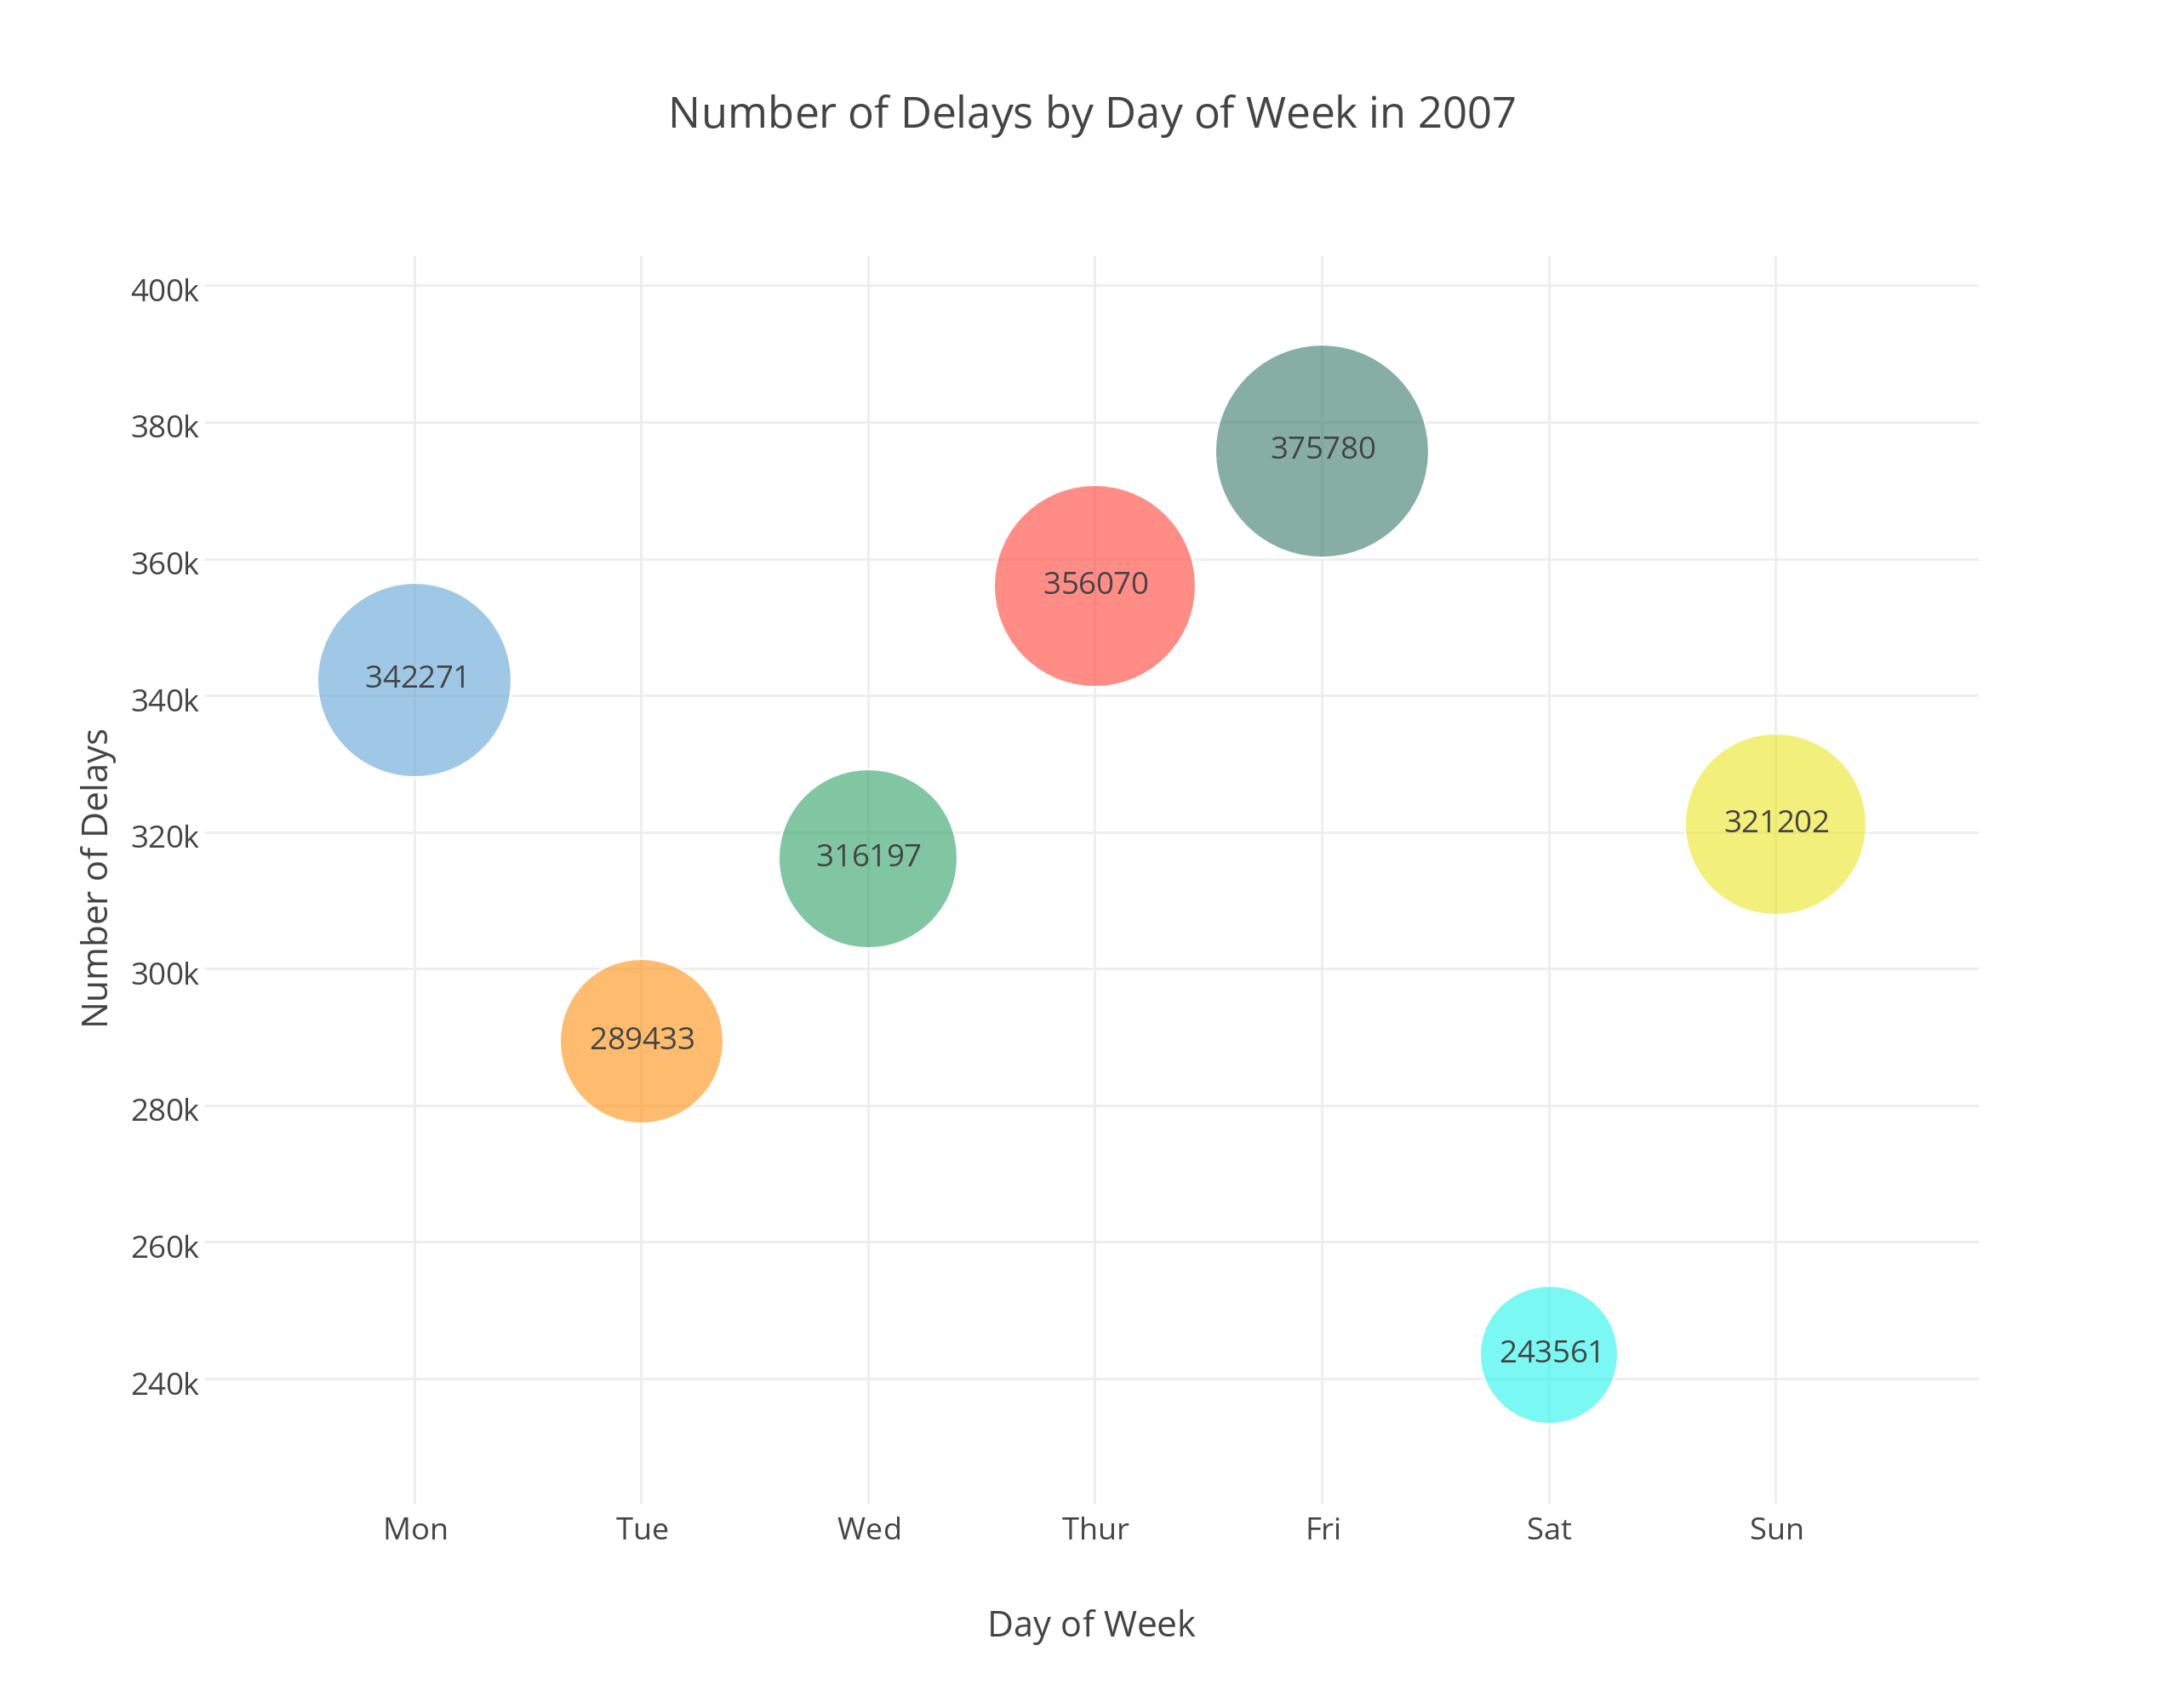
\includegraphics[width=1.1\linewidth]{delayedbyweek.png}
\caption{Chart of Delays by Day of Week}
\label{fig:weekdelays}
\end{figure}

\begin{figure}[htb]
\centering
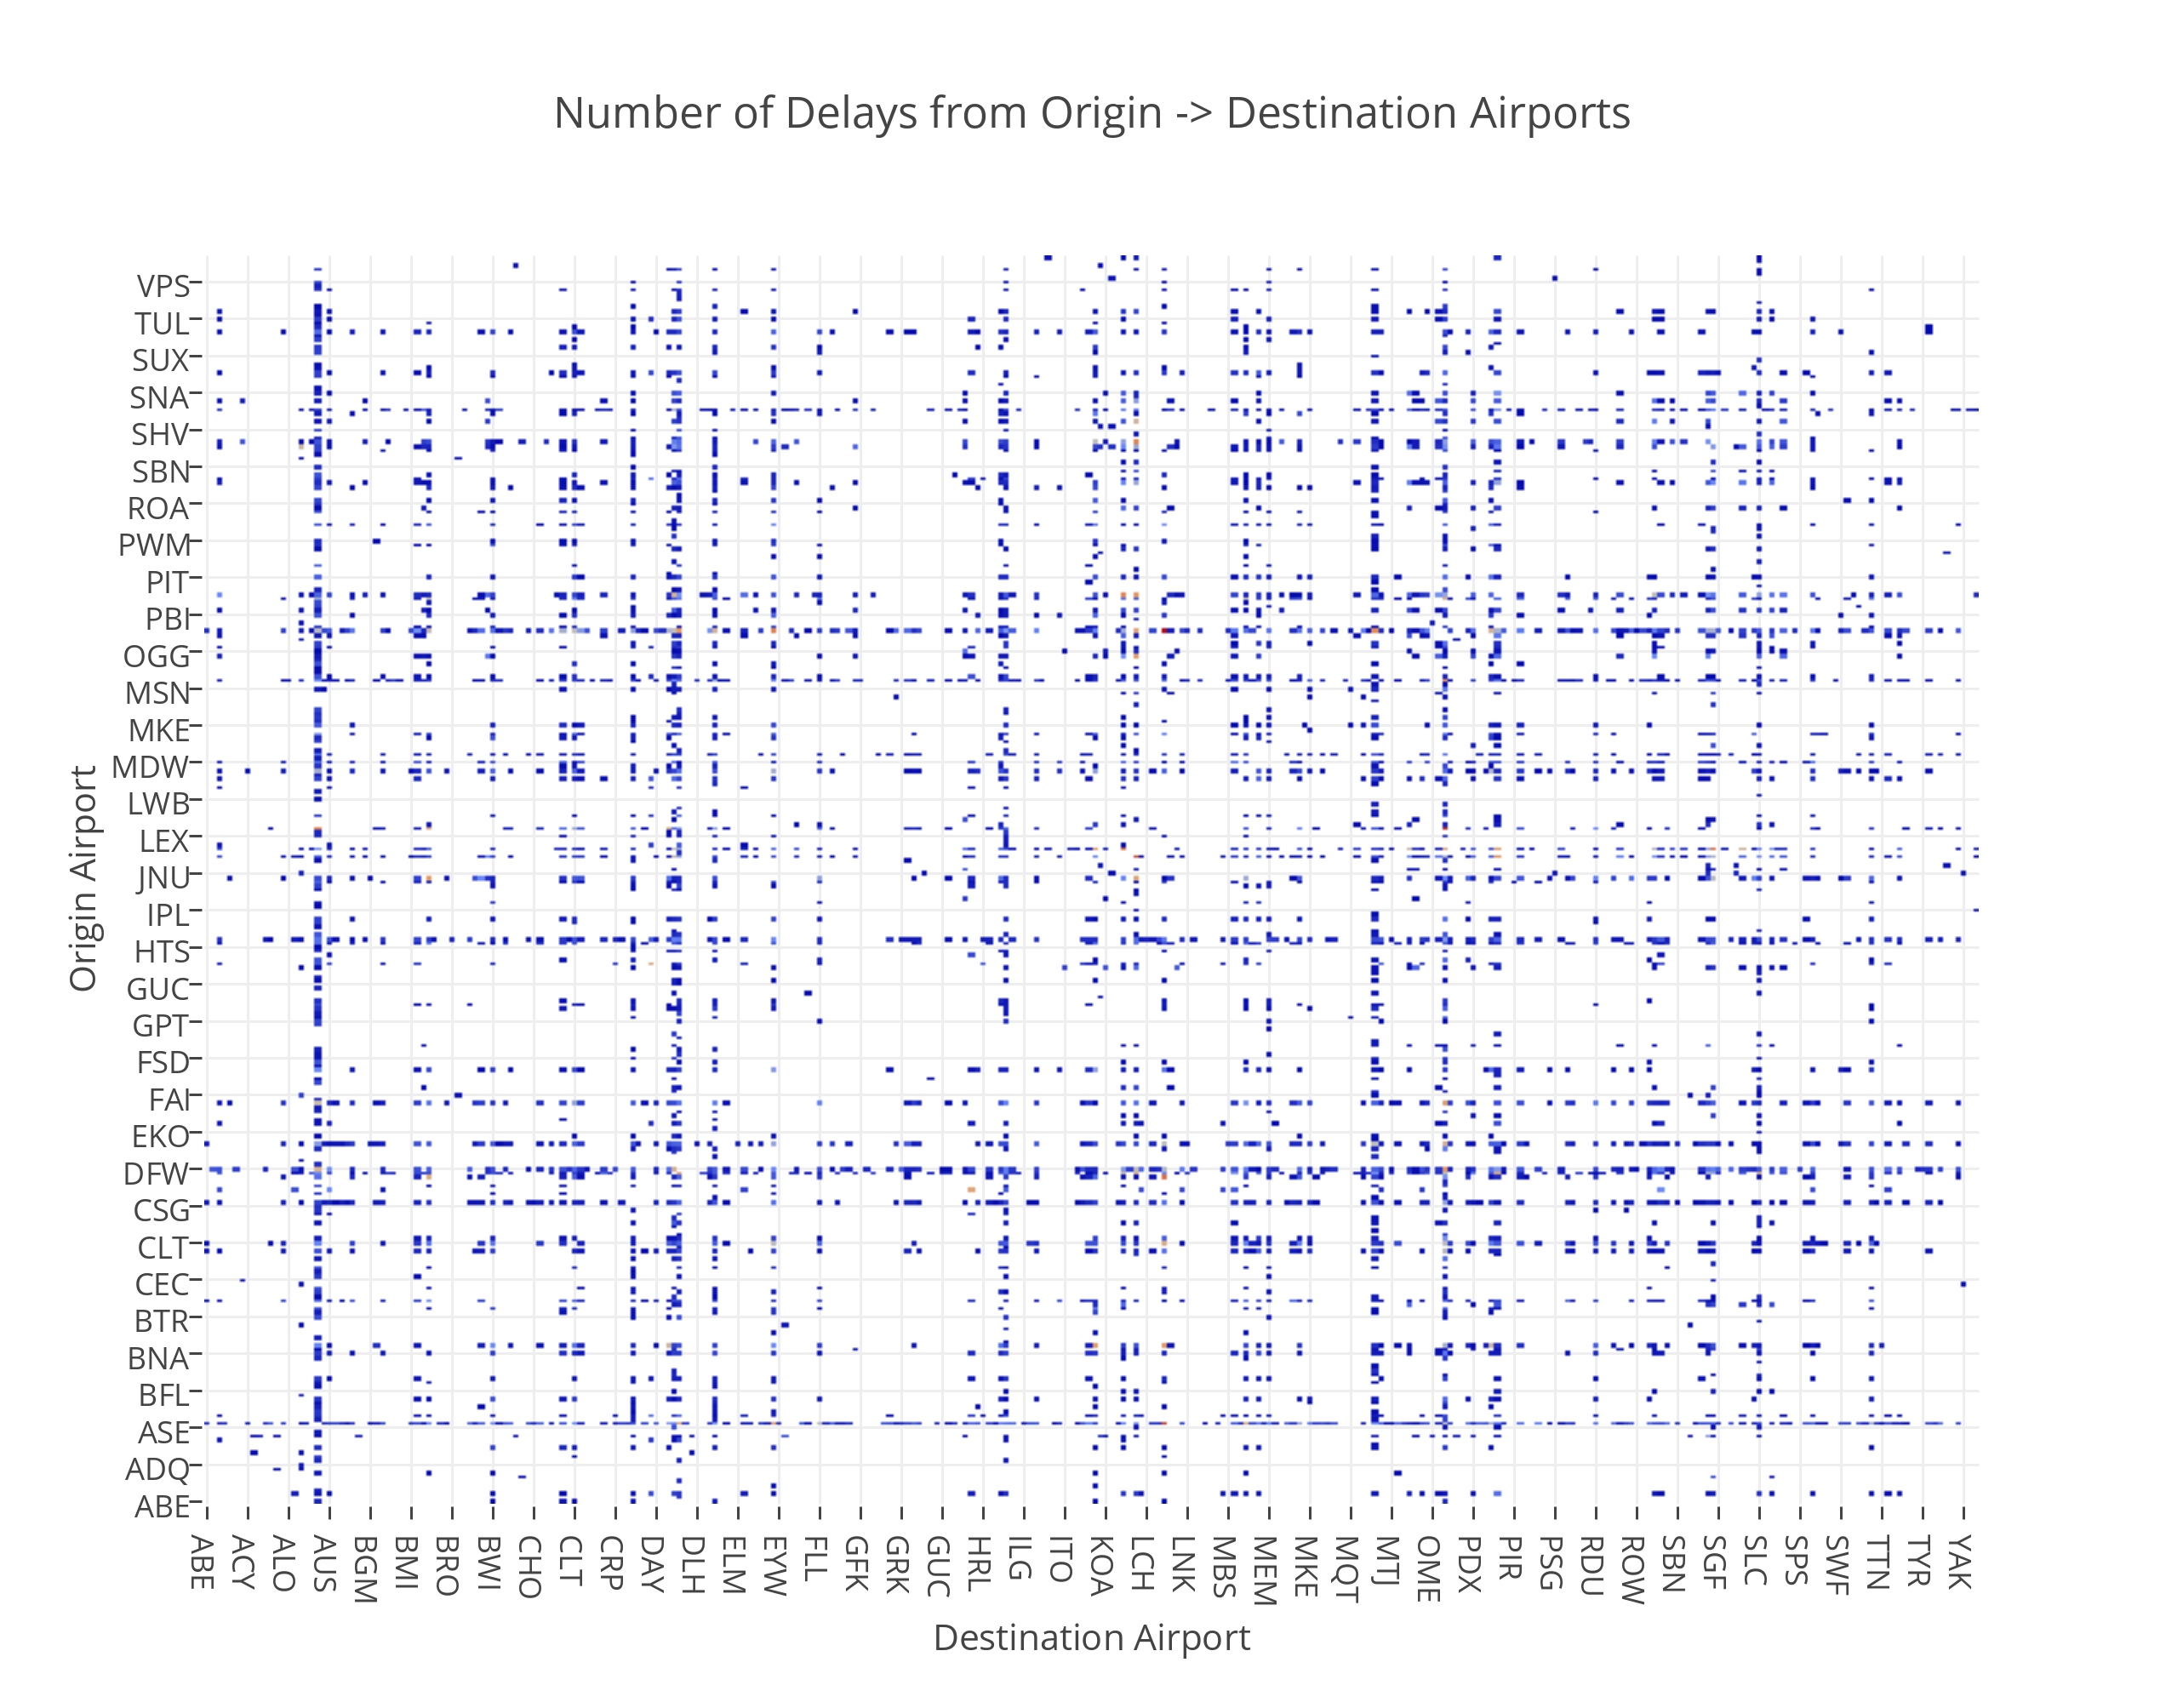
\includegraphics[width=1.1\linewidth]{heatmap.png}
\caption{Star chart of delays from origin to destination airports}
\label{fig:heatmap}
\end{figure}

\section{Predicting Flight Delays}
This section describes the workflow we used to predict flight delays. The flight delays were predicted via a sliding window, beginning with one day's worth of flight data (20 000 records). The window size is slowly increased to 5 million records, which is 80\% of the dataset, by an increment of about 20 000 records. This sliding window is suitable for such a time-series data to simulate real-time prediction, in which we have a certain number of previous day's worth of records and have to predict the flight delay on the current query flight. 

We used python and scikit-learn for classification and prediction. For visualisation, we used Plot.ly and matplotlib libraries. In order to process the huge dataset, we used Hadoop's map-reduce framework with multiple mappers and one reducer on the school's Tembusu Compute Cluster. 

\subsection{Overview}
Figure \ref{fig:overview} shows a graphical flow of our data mining pipeline. 

The raw flight data is first combined with weather data obtained from NOAA and flight distances calculated from the latitude and longitude of the origin and destination airports. The merged dataset is then preprocessed for feature agglomeration for better representation of the data. In our pipeline, we make use of the map-reduce architecture. The mappers will perform find k-Nearest-Neighbours to the query flight among the $n$ training examples they receive. Then, they will train a classifier on the k-nearest-neighbours. This project explored various classifiers. The mapper outputs the actual and predicted classification of delay. One reducer collects all the classification labels and calculates the result statistics for the dataset. 

We perform a sliding window classification for this time-series data. We iterate through the window size $n$ from 20 000 data records, which represent the number of flight data from one day, to 5 million records, or 80\% of the dataset. Each increment consists of 1 day's worth of flight data, around 20 000 records. 

\begin{figure}[htb]
\centering
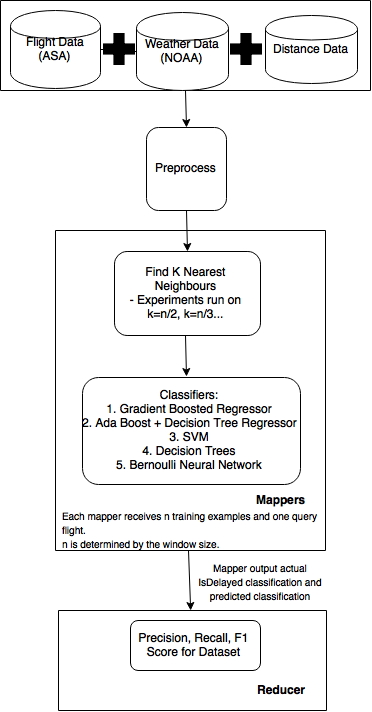
\includegraphics[height=1.3\linewidth]{CS5228-final2.png}
\caption{Overview of prediction pipeline}
\label{fig:overview}
\end{figure}

\subsection{Preprocessing}
\subsubsection{Combining weather and distance data}
The first step of the preprocessing pipeline is to combine the raw flight data with weather data. The weather data is obtained from NOAA in a summary of meteorological data obtained from the airport weather station. The average meteorological data of each day over the Years 2007 and 2008 is obtained and merged with the flight data. There are two main problems in these datasets which require some data clean-up: missing data and inaccurate data. Some airports do not have weather stations or may not report a certain data field, which results in missing data. In the case where data from other airports in the state are present, we use the mean of the state. Where the mean of the state is not available, we use the mean of all the airports in USA. In cases where we can intelligently guess, we will fill in the data fields with our external knowledge. For example, McCarran International Airport (LAS) does not report precipitation data. As we know LAS is situated in Las Vegas which is a very dry state, we fill in the precipitation as 0 mm, since the place is generally known to be desert-like. On inaccurate data, we will remove the data field and attempt to fill it up as per missing data, i.e. mean of state. Santa Barbara Airport (SBA) has no temperature readings but reported maximum and minimum temperatures as -9999.0. This messes up the dataset and is therefore removed. 

After this, we combine the flight data with the data on the distances between the origin and destination airports. We obtain the latitude and longitude coordinates of the two airports and estimate the flight distance using the haversine formula, factoring in the radius of the Earth (est. 6373km).

\begin{multline}
\scriptstyle \text{haversin}(\theta)=\sin^2\left(\frac\theta2\right)=\frac{1-\cos(\theta)}2, \\
\scriptstyle d=2r\sin^{-1}\left(\sqrt{\text{haversin}(\phi_2-\phi_1)+\cos(\phi_1)\cos(\phi_2)\text{haversin}(\lambda_2-\lambda_1)}\right)
\end{multline}

Where $\phi_1, \phi_2$ is the latitude of points 1 and 2, $\lambda_1, \lambda_2$ for the longitude of points 1 and 2, $r$ radius of the sphere and $d$ the distance that we want to find.

We believe flight distance do affect the length of flight delays, because in general, insurance companies give greater financial compensation for long-haul flights than shorter flights for the same amount of delay.

\subsubsection{Feature selection}
After the data is combined, we merge certain columns to better represent the data. We first merge the columns of Arrival Delay, Departure Delay, Carrier Delay, Security Delay, Weather Delay, Security Delay and Late Aircraft Delay to a column called Total Delay. Then we formulate a column IsDelayed as a boolean which is true of the Total Delay is greater than 15 minutes and false otherwise. We merge the Year, Month, Day, Departure Time into a column called DateTime, then sort the data by the DateTime. We also calculate the days from nearest American public holiday such as Christmas or New Year. This is because there tend to be more flights nearer such dates and the airports will get more congested which could result in more delays. Lastly, we convert all the nominal data columns to numeric ones to facilitate classification. 

\subsection{kNN and Classifers}
The parameter $k$ in k-Nearest-Neighbours is defined as a proportion of the window size. We define $k=n/2$, $k=n/3$ and so forth, so that each run of the dataset has the same proportion of neighbours. 	
The flights from the result of the k-Nearest-Neighbours are put through various classifiers: Gradient Boosted Regressor, Ada Boost and Decision Tree Regressor, Support Vector Machines, Decision Trees and Bernoulli Neural Networks. These classifiers are obtained from the scikit-learn package and their default settings are used, as the focus of the project is to explore the effect of window size rather than classifier parameters. 

\subsection{Validating the Results}
We validate the results by calculating the precision, recall and fscore for each predicted set as compared to the actual dataset. This is done using the scikit-learn API. In our situation, we prefer a lower recall rate to a higher precision. False negatives is favoured over false positives. From a consumer point of view, it is better to anticipate a flight delay than to be delayed. When a flight delay is anticipated, alternative transport routes or plans can be made. The passenger can prepare to take a later connecting flight, and it is in his favour that the flight lands on time. However, if the flight is delayed when our prediction algorithm reports otherwise, the passenger miss the connecting flight or  appointments. 

\subsection{Map-Reduce} 
We made use of Hadoop on the Tembusu Computer Cluster, which is run on Linux, to parallize the classification process in order to speed up computation. With Hadoop, iterating through the entire 7.5 million dataset with a window size of 20 000 takes roughly 2 minutes for the Gradient Boosted Regressor. A full iteration from 1 day worth of training data record to 5 million training records took over 8 hours. Other classifiers, however, took different amounts of time. Our map-reduce stack is implemented with multiple mappers and one reducer. 
\subsubsection{Mapper}
As we are performing a sliding window over the time-series data, each mapper only needs to know the $n$ training data and the one query flight. The training data contains of the past $n$ records of flight data, which ranges from one day worth of records (20 000) to 5 million, with an increment of a day at each iteration. The mapper will find k-nearest-neighbours to the query flight from the training data, where $k$ is a proportion of $n$. Then it will classify the k-neighbours using one of the classifiers and output the actual classification label and the predicted classification label. 

\subsubsection{Reducer}
There is only one reducer in each run of the dataset. The reducer takes in the actual classification label and predicted classification label and outputs the precision, recall and F-score for the $n$ and $k$ parameters. 

\section{Results}
We ran a binary classification prediction problem. Given a window size $n$ training flights, we want to classify whether the query flight will be delayed or not. We ran this over several classifiers and regressors. The regressors will output an estimated number of minutes of delay for the query flight, in which we classified the flight to be delayed if the estimation were above 15 minutes, and not delayed otherwise. 

We varied the number of nearest neighbours, $k$ as a fraction of $n$. For each $k$, we ran the algorithms from $n = 20 000$ to $n = 5 000 000$, each time increasing $n$ by 20 000. These numbers are chosen because 20 000 is the average number of commercial flights per day and 5 000 000 comprises of 80\% of the flights. Hence, we create a window consisting of the flight for a single day to 80\% of the flight data given, each time increasing the number of training data by the number of flights per day. We term one full run as running through $n = 20 000$ to $n = 5 000 000$ for one $k$. 

For the algorithms, we used Gradient Boosted Regressor (GBR), Ada Boost with Decision Tree Regressor, (ADR) Support Vector Machines (SVM), Decision Trees (Tree) and Bernoulli Neural Networks (BNN), with their default parameters. 

The Tables \ref{table:k/2} and \ref{table:k/3} shows the average precision, recall and f-score for each algorithm ran. 

% Add some graphs
\begin{figure}
\centering
\begin{minipage}{.45\linewidth}
  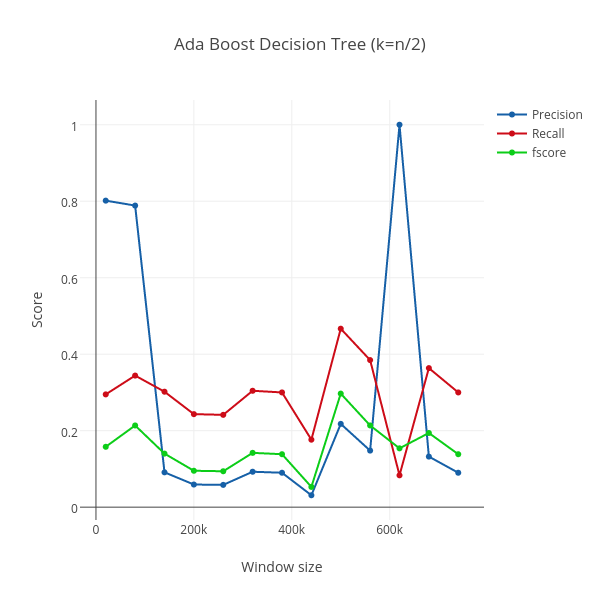
\includegraphics[width=\linewidth]{../data_mapred/img/truncated/adr2.png}
  \label{fig:adr2}
\end{minipage}
\begin{minipage}{.45\linewidth}
  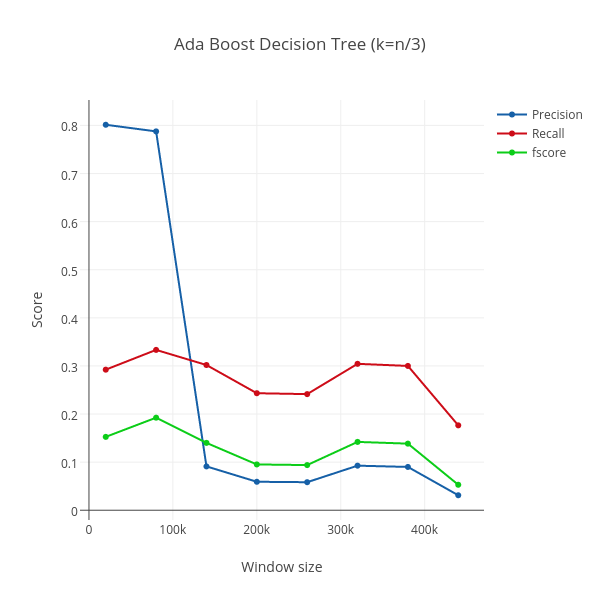
\includegraphics[width=\linewidth]{../data_mapred/img/truncated/adr3.png}
  \label{fig:adr3}
\end{minipage}
\begin{minipage}{.45\linewidth}
  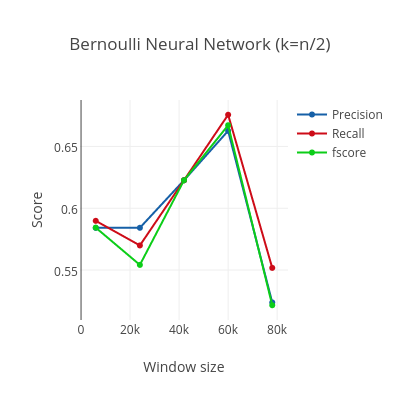
\includegraphics[width=\linewidth]{../data_mapred/img/truncated/bnn2.png}
  \label{fig:bnn2}
\end{minipage}
\begin{minipage}{.45\linewidth}
  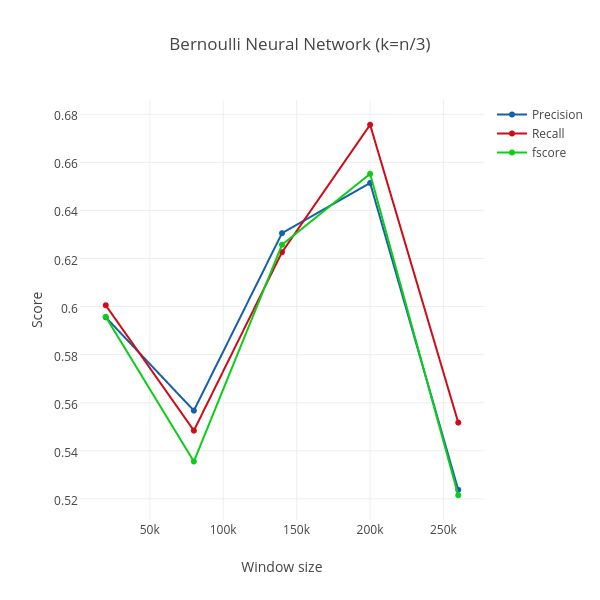
\includegraphics[width=\linewidth]{../data_mapred/img/truncated/bnn3.png}
  \label{fig:bnn3}
\end{minipage}
\begin{minipage}{.45\linewidth}
  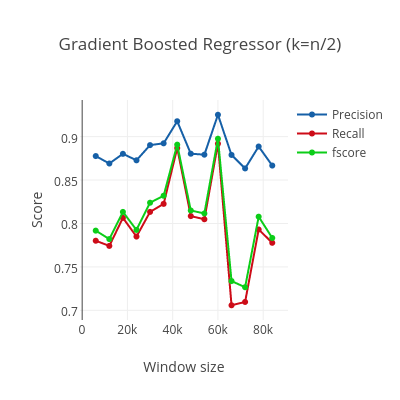
\includegraphics[width=\linewidth]{../data_mapred/img/truncated/gbr2.png}
  \label{fig:gbr2}
\end{minipage}
\begin{minipage}{.45\linewidth}
  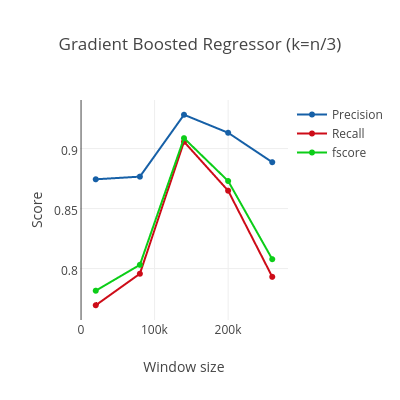
\includegraphics[width=\linewidth]{../data_mapred/img/truncated/gbr3.png}
  \label{fig:gbr3}
\end{minipage}
\begin{minipage}{.45\linewidth}
  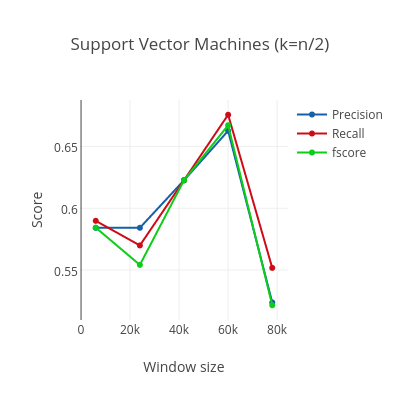
\includegraphics[width=\linewidth]{../data_mapred/img/truncated/svm2.png}
  \label{fig:svm2}
\end{minipage}
\begin{minipage}{.45\linewidth}
  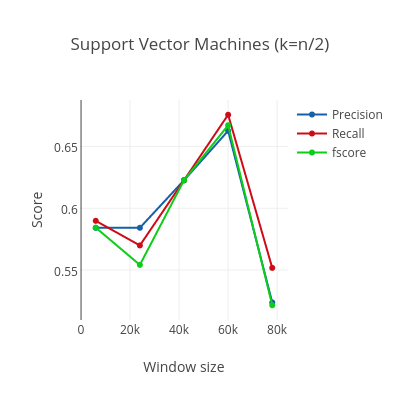
\includegraphics[width=\linewidth]{../data_mapred/img/truncated/svm2.png}
  \label{fig:svm3}
\end{minipage}
\begin{minipage}{.45\linewidth}
  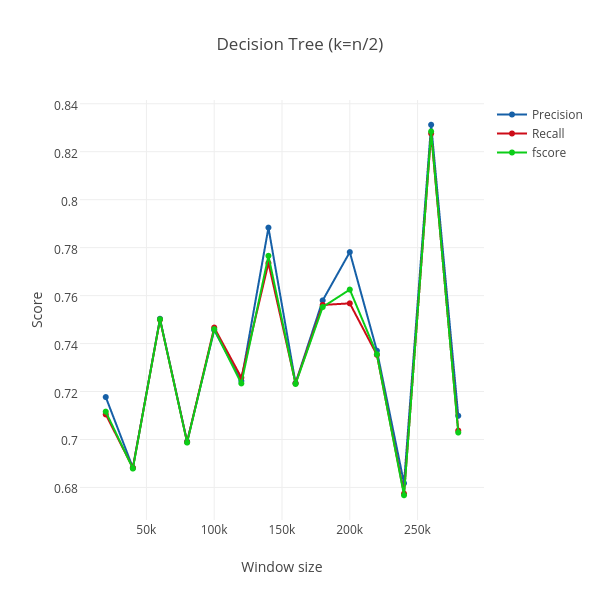
\includegraphics[width=\linewidth]{../data_mapred/img/truncated/tree2.png}
  \label{fig:gbr2}
\end{minipage}
\begin{minipage}{.45\linewidth}
  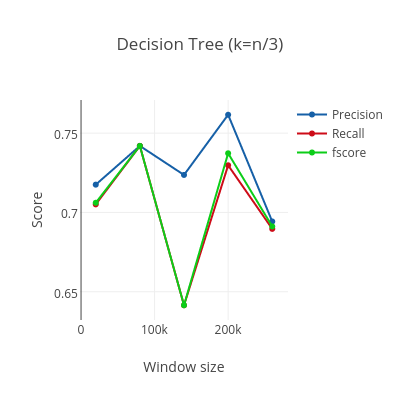
\includegraphics[width=\linewidth]{../data_mapred/img/truncated/tree3.png}
  \label{fig:tree3}
\end{minipage}
\caption{Scores for regressors with different window sizes.}
\label{fig:adr}
\end{figure}

% score table
\begin{centering}
\begin{table}
\begin{tabular}{ | l | l | l | l | l | l | l |}
  \hline
   & \textbf{GBR}& \textbf{ADR} & \textbf{SVM} & \textbf{Tree} & \textbf{BNN}\\ \hline
  \textbf{Precision} & 0.82 & 0.24 & & 0.83 & 0.45\\  \hline
  \textbf{Recall} & 0.66 & 0.29 & & 0.81 & 0.50\\  \hline
  \textbf{F-Score} & 0.69 & 0.20 & & 0.80 & 0.45\\  
  \hline
\end{tabular}
\label{table:k/2}
\caption{Average scores for $k=n/2$}
\end{table}
\end{centering}

\begin{centering}
\begin{table}
\begin{tabular}{ | l | l | l | l | l | l | l |}
  \hline
   & \textbf{GBR}& \textbf{ADR} & \textbf{SVM} & \textbf{Tree} & \textbf{BNN}\\ \hline
  \textbf{Precision} & stuff & 0.25 & & Test & \\  \hline
  \textbf{Recall} & stuff & 0.27 & & Test & \\  \hline
  \textbf{F-Score} & stuff & 0.16 & & Test & \\  
  \hline
\end{tabular}
\label{table:k/3}
\caption{Average scores for $k=n/3$}  
\end{table}
\end{centering}

\subsection{Effect of Different Algorithms}
Tree-based classifiers such as Decision Tree Classifier, Ada Boosted Regressor and Gradient Boosted Regressor classified the data very quickly. Running for one window size through the entire dataset took around 30 minutes. For one full run of varying window size with a fixed proportion of $k$ neighbours, these classifiers took 8 hours to two days to classify the data. Classifiers such as SVM and Neural Networks have been known not to scale very well to this large dataset, and they took more than six days for one full iteration. 

A simple decision tree classifier performed best, yielding 83\% precision and 80\% recall, followed by the gradient boosted regressor. The Ada Boost performed worst with a precision of 24\% and the neural network also fell below 24\%. 

\subsection{Effect of Window Sizes}
In general, the smaller the window size yielded better results. This shows that the most recent flight data is most useful in predicting whether the query flight will be delayed. Hence, programs and sites which do flight delay prediction may reduce space complexity by not needing to store too many flights. 

\subsection{Effect of k}

\subsection{Feature Selection} 
At best, the classifiers reported results of about 83\% precision. This shows that the algorithm chosen has lesser importance as compared to the feature selection. To achieve good prediction results with this dataset, we need to pick out the salient features for classification. We tested a dataset without distance data with the Gradient Boosted Regressor, and the dataset had slightly lower precision of 80\% as compared to 82\% with distance as a feature. This shows that the distances of flights do make a difference in prediction of delays. 

As compared to the literature where no additional data is merged into the flight data, our method achieved a performance of 10\% better precision. The additional features of weather and distances are useful in determining the possibility of delay of the flight. Our results are on par with commercial flights delay sites and literature. 

\section{Further Work}
Much can be done to explore the effect of varying window size with the accuracy of predicting flight delays: different sizes of $k$, constant $k$ with varying window size, different classifiers, different classifier parameters, and even different window size and window increment sizes. One might want to look into kernel methods that scale for using kernel-based classifiers such as SVM for classifying such a huge dataset. 

One can also explore which features are most useful in flight delay prediction. This would be done using logistic regression of each feature versus the delay vector. However, logistic regression on such a scale is very slow. An experiment that we ran involved a logistic regression of maximum temperature vs number of minutes of delay, which fitting the data to the logistic regressor took more than a day, and the reported correlation value was only about 0.2. 

One can also explore using the full dataset of flights from 1987 to 2008 with weather data. However, NOAA only provides weather data from 1900 onwards, so one has to disregard weather data from Years 1987 to 1900. To do such an experiment, one needs to come up with a more efficient way of scaling the experiment, with a variation of our map-reduce architecture.

\section{Conclusion}
This project explored a binary classification prediction problem with data from commercial flights within America in Year 2007, consisting of 7.5 million records. The raw flight data is merged with weather data from NOAA and flight distance data calculated from the latitude and longitude of airports. Sliding window experiments were run the past $n$ flights picked out as training data for the query flight. A k-nearest-neighbours classification was done with $k=n/2$ and $k=n/3$. With several regressors and classifiers on a map-reduce architecture on the Tembusu Compute Cluster, our method reported an average precision of 83\% at best, which is on par with commercial sites and better than some literature. 

\bibliography{cs5228.bib}
\bibliographystyle{aaai}

\end{document}
